

\subsection{PDSurvey Platform}

	The architecture for the public disply survey (PDSurvey) platform can be split into three main sections (see Figure \ref{fig:4-pdsurvey-platform}). 

	\begin{itemize}
	\item \textbf{PDAdmin}: 
	\item \textbf{PDServer}: 
	\item \textbf{PDClient}:
	\end{itemize}

	\begin{figure}%[btph]
	    \begin{center}
	        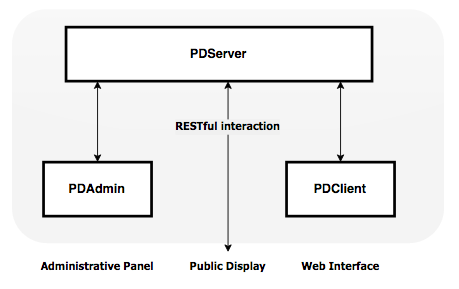
\includegraphics[width=.7\columnwidth]{img/4_implementation/4-overview}
	    \end{center}
	 \caption[Overview of the PDSurvey platform]{Overview of the PDSurvey platform: (a) PDServer containing the Node.js server, (b) PDBackend the Angular.js frontend for administrators and (c) PDClient the interface included on public displays and optimized for mobile devices.}
	 \label{fig:4-pdsurvey-platform}
	\end{figure}



	\begin{enumerate}
	\item begin with describing what the platform does, which views it has (show screenshots).
	\item describe the client
	\end{enumerate}



	\subsubsection{PDAdmin}

		For administrative purposes we created an interface, enabling display providers to create, manage and distribute surveys to public displays. 

		% admins
		Display providers have the ability to create their own questionnaires or to select from a list of standardized questionnaires (introduced in section \ref{sec:questionnaires}).


		% normal process


		% Wizard

		% eigene Module
			advancing > modular aufgebaut

			% SCREENSHOT: Wizard
			% SCREENSHOT: individually accessing 1 Display / 2 Surveys / 3 Campaigns
			% SCREENSHOT: Dashboard

		All data and actions get transmitted to the server via HTTP request/response calls.

	\subsubsection{PDServer}

		PDServer makes a relatively simple impression. It consists of a Node.js server, which to the outside only acts as a REST server. Processing REST calls, performing CRUD operations and responding with JSON objects. Besides this REST functionality a rudimentary authentication mechanism is already implemented on the server and the capability for further logic, determining which client should ask which question next. This functionality might become of interest when trying to spread standardized questionnaires of longer length across multiple users or multiple displays. It would be intended for the server to keep track which questions have already been answered and to tell each instance of PDClient which question to ask next, in order to achieve a balanced question profile.

		% Mongoose maintians the object models and performs all CRUD applications on MongoDB 
		%  >> don't get too technical!!

		The specification of PDServer's REST API can be found in the documentation (see Appendix \ref{appendix:documentation}).



	\subsubsection{PDClient}

		Our client tool was kept as simple and minimalistic as possible. It is running on a completely different code base than PDBackend, the only communication between the two is via REST, exchanging JSON objects.

		
			Goal: reduce logic and complexity on client-side. The client either receives all questions for the questionnaire (caching-ability), or it always only loads the next question on-demand. For this purpose the REST interface provides the /nextQuestion API.
		
			% Optional: campaign specific view

		Overview of elements:

		\textbf{Survey page}: all questions are loaded at once on initial startup, then one question gets displayed at a time. Settings for the survey can be modified in the PDBackend (e.g. number of questions to display, duration of the survey, ...). Once the user makes a choice, it is directly logged on the server. In case that a participant aborts answering the survey, the questions answered so far are still recorded.

		\textbf{About page}: giving information about the research project. Some people are sceptical and have doubts 

		\textbf{Welcome page} (to teaser people to participate). It turned out that a significant larger number of people were willing to participate in a survey, after knowing that it doesn't take long, is university-related and for what it will be used for. These arguments were amongst others stated in semi-structured interviews during the field study.





	\subsubsection{EmbedCode}

		The embed code, JavaScript Code Injection, turned out to be a pure proof-of-concept, since it was not needed for the field study at the university. The problem was that the application on which PDSurvey should be integrated did not support any HTTP calls, thus we had to fall back on another solution. This embed code was intended to be used by display operators, wanting to include optional questionnaires hovering over their normal application. 

		% also show the mockup / technical demonstration of the JavaScript embed code. It was a proof-of-concept, demonstrating the feasibility of embedding questionnaires as an overlay (additional DIV layer), injected via one (minified) line of Javascript. 

		% -Solutions: (pdsurvey/public/tracking/survey.js bzw. testing/tracking-code/index.html)

		% Use Case
		An example use case is exemplified here ...


		% Implementation

		The implementation is quite simple. 
		 - giving one unique line of JavaScript code to the display provider
		 - add it to the end of the HTML body tag
		 - this minified one-liner adds a HTML script-tag to the DOM,
		 - loading a personalized JavaScript file from the PDBackend
		 - jQuery and/or Angular.js get loaded asynchronously
		 - a copy of PDClient gets dynamically built on client side
		 - all questions for the questionnaire get loaded via REST API from the server
		 - and the responses get sent back to the server for logging

		Useful links can be found here:

		\url{https://developers.google.com/analytics/resources/concepts/gaConceptsTrackingOverview}

		\url{http://en.wikipedia.org/wiki/Web_bug}

		\url{http://stackoverflow.com/questions/3534524/how-does-the-embedded-google-analytics-javascript-work}


	\subsubsection{Future Work}

		% what is still missing

		Authentication: using passport, HTTPS was not offered in the beginning. As of now it is not needed, since we only had one client. All REST Update and Delete functionality was restricted to the URI of the PDServer, which is also the desired approach in the production setting.

		Evaluation of results: dynamic queries, information visualization

